\chapter{Theory}
\label{chap:theory}

\section{2D Image Processing}

Image processing describes the application of different algorithms on images with the purpose of gaining certain information about it or changing its representation. Most of the time images are given as two dimensional pixel arrays where each entry denotes the intensity of that pixel. In the case of grayscale images the value is between 0 and 255 representing black and white respectively. When handling color images an additional 3rd dimension is added with three channels representing a red, green, blue (rgb) encoding. Each entry, again, has values between 0 and 255 representing color intensity. \\
Instead of imagining an image as a flat 2D object, it can also be seen as a terrain with surface, where the height of each coordinate is determined by the intensity of its value. An example of this is shown in figure \ref{fig:image_surfaces}. 


\begin{figure}[!htb]
	\centering
	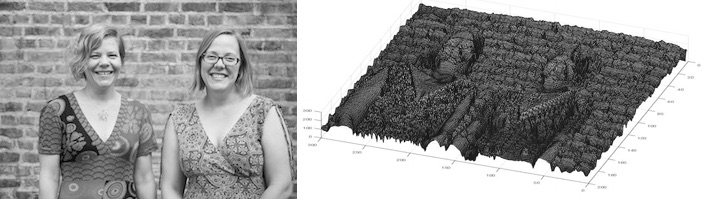
\includegraphics[width = 0.9\textwidth]{images/image_surfaces.jpg}
	\caption{Left: image represented as 2D flat surface. Right: image as 3D terrain with uneven surface. \protect\footnotemark}
	\label{fig:image_surfaces}
\end{figure}

\footnotetext{Figure taken from \url{https://plus.maths.org/content/fourier-transforms-images}}

%TODO how does this work for color images?
%-> see scaling the scattering transform

Like every other surface, these images can now be approximated as the sum of many different two dimensional sine waves. 2D sine waves are defined as in equation \ref{eq:2d_sine}, where f $a$ is the amplitude and $h, k$ are the frequencies in $x$ and $y$ direction respectively.

\begin{equation}
	f = a \sin(h\cdot x+k\cdot y)
	\label{eq:2d_sine}
\end{equation}

To give an example of how this approximation looks like, figure \ref{fig:2d_sine} shows examples of three different two dimensional sine waves. It can be observes that higher amplitudes dominate the resulting wave, i.e. determine the direction of the wave stronger than the smaller amplitudes. 


\begin{figure}[!htb]
	\centering
	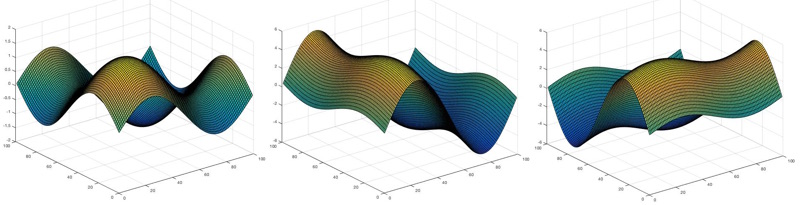
\includegraphics[width = \textwidth]{images/2d_sine.jpg}
	\caption{Left: $\sin(x) +\sin(y)$. Middle:  $5 \sin(x)+ \sin(y)$. Right: $	\sin(x)+5\sin(y)$. On the middle and right images the higher amplitudes of 5 dominate the resulting wave. \protect\footnotemark}
	\label{fig:2d_sine}
\end{figure}

\footnotetext{Figure taken from \url{https://plus.maths.org/content/fourier-transforms-images}}

\section{Fourier Transformation}

A Fourier Transform (FT) decomposes a signal into the frequencies that make it up.
\subsection{One dimensional FT} 

In the case of one dimensional signals the decomposition are the coefficients of the sine waves representing the signal. A good example of this would be the decomposition of a  The FT is defined by equation \ref{eq:forward_FT} for any real number $\omega$ and any integrable function $f:\mathbb{R} \rightarrow \mathbb{C}$. 

\begin{equation}
	\tilde{f}(\omega) = \int_{-\infty}^{\infty} f(x)\ e^{-2\pi i x \omega}dx
	\label{eq:forward_FT}
\end{equation} 

To get back to the Fourier domain when the given a frequency, the inverse Fourier transform defined in equation \ref{eq:inverse_FT} is used.  \\

\begin{equation}
	f(x) = \int_{-\infty}^{\infty} \tilde{f}(\omega)\ e^{2 \pi i x \omega}d\omega
	\label{eq:inverse_FT}
\end{equation}

When using discrete instead of continuous functions, the integrals in the definitions become sums. Then the definition of the forward FT is given in equation \ref{eq:forward_FT_dis} and in equation \ref{eq:inverse_FT_dis} for the inverse FT. 

\begin{equation}
\tilde{f}(\omega) = \sum_{x=1}^{n} f(x)\ e^{-2\pi i x \omega}
\label{eq:forward_FT_dis}
\end{equation} 

\begin{equation}
f(x) = \sum_{x=1}^{n} \tilde{f}(\omega)\ e^{2 \pi i x \omega}
\label{eq:inverse_FT_dis}
\end{equation}

\subsection{Two dimensional FT}

Since images are two dimensional objects the Fourier transform needs to be extended. The Fourier transform then becomes a complex function of two or more real frequency variables $\omega_1, \omega_2$. Since images images are finite objects the discrete version of the two dimensional Fourier transform is given in equation \ref{eq:forward_FT_2D} for the forward case and in equation \ref{eq:inverse_FT_2D} for the inverse case.

\begin{equation}
	\tilde{f}(\omega_1, \omega_2) = \sum_{x=1}^{n} \sum_{y=1}^{m} f(x,y)\ e^{-2\pi i (\omega_1 \cdot x + \omega_2 \cdot y)}
\label{eq:forward_FT_2D}
\end{equation}

\begin{equation}
f(x, y) = \sum_{x=1}^{n} \sum_{y=1}^{m} \tilde{f}(\omega_1, \omega_2)\ e^{2\pi i (\omega_1 \cdot x + \omega_2 \cdot y)}
\label{eq:inverse_FT_2D}
\end{equation}

\section{Scattering Transform}

A transformation from the Fourier to the frequency domain cannot only be performed by using the sine but in principal with any given periodic function.
Wavelets are wave-like oscillation with an amplitude that begin and end at zero. In most use cases wavelets are specifically crafted to have certain properties. 
The Scattering Transform is based on a Morlet wavelet, which is defined in equation \ref{eq:morlet2d}.

\begin{equation}
	\psi(u) = C_1 (e^{iu.\xi} - C_2) e^{\frac{-|u|^2}{2\sigma^2}}
\end{equation}

%TODO: what is the meaning of all those symbols?

where $C_2$ is chosen such that $\int \psi(u) du = 0$. $u.\xi$ denotes the innerproduct of $u$ and $\xi$ and $|u|^2$ is the norm in $\mathbb{R}^2$. 
%TODO: what is sigma
%TODO: what is xi
%TODO: what is C_1 and C_2
Figure \ref{fig:morlet2d} shows the 2 dimensional Morlet wavelet with parameters $\sigma = 0.85$ and $\xi = \frac{3\pi}{4}$. These parameters are taken from \cite{scatteringTransform2012}. No additional fine tuning is done in this work. 

\begin{figure}[!htb]
	\centering
	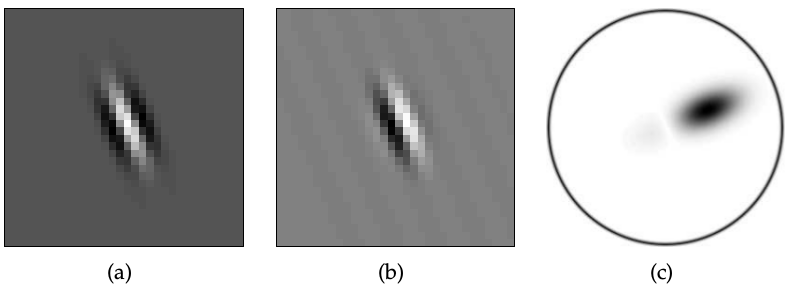
\includegraphics[width = 0.9\textwidth]{images/morlet2d.png}
	\caption{Complex morlet wavelet. a) Real part of $\psi$. b) Imaginary part of $\psi$. c) Fourier modulus $|\hat{\psi}|$. Image taken from \cite{scatteringTransform2012}.}
	\label{fig:morlet2d}
\end{figure}

\subsection{Properties of the Scattering Transform}

%TODO: How detailed? Just hint at it or copy entire section of original paper?

As already pointed out in the introduction, key properties of object detection are invariance with respect to scale, rotation, localization and deformation. The Scattering transform extends a simple 2D Fourier transform in exactly these properties. The Fourier transform is translation invariant, but unstable with respect to deformations at high frequencies. This implies that the representation is also unstable with respect to deformations.
Additionally a Fourier transform loses to much information. Two different signals can have Fourier transforms with exactly the same moduli. \\

A wavelet, in comparison to the sinusoidal waves of the Fourier, is a localized waveform and therefore stable with respect to deformation. 


\section{Convolutional Neural Networks}

%TODO

For most image-related tasks, i.e. classification or object detection, a picture is used as a collection of pixels. However, not all pixels are equally important and subsets of the entire image form meaningfully connected subcollections. This might be a face in a photo of a family gathering. For humans the ability to detect these features and contextualize them comes naturally, for computers it does not. Therefore convolutional neural networks (CNNs) are used. Convolutions are essentially just the application of filters on an image. The filter is applied at every possible location in the image, as described in figure: 

%TODO: image for filter fig

In CNNs there are multiple stages of filters in sequential order and multiple filters per layer. That means at every stage of the network different filters are applied on the outcome of an earlier step. The filters are assumed to learn different features of the images. The later the stage, the higher the level of complexity of the feature to be learned. That means, that an early filter might learn simple attributes such as edges or colors while a later filter might learn 

%QU: allowed to reference link to guide?


